\chapter{Enterprise Java Beans}
Enterprise Java Beans (EJBs) sind serverseitige Java-Komponenten die Business Logik implementieren. In einem Flugbuchungssystem wären typische Business-Methoden \verb|bookFlight| oder \verb|payFlight|. EJBs vereinfach in der Regel die Entwicklung von grossen und verteilten Applikationen. Die Beans laufen innerhalb eines Container, welcher System Services zur Verfügung stellt, wie das Tansaktionsmgmt. oder Sicherheitsautorisierungen. Es wird klar getrennt zwischen View und Logik, in den Beans kann nur Logik implementiert werden. Zudem kann der Applikationsassemblierer neue Applikationen aus existierenden Beans zustammenstellen.

\begin{figure}[h!]
	\centering
	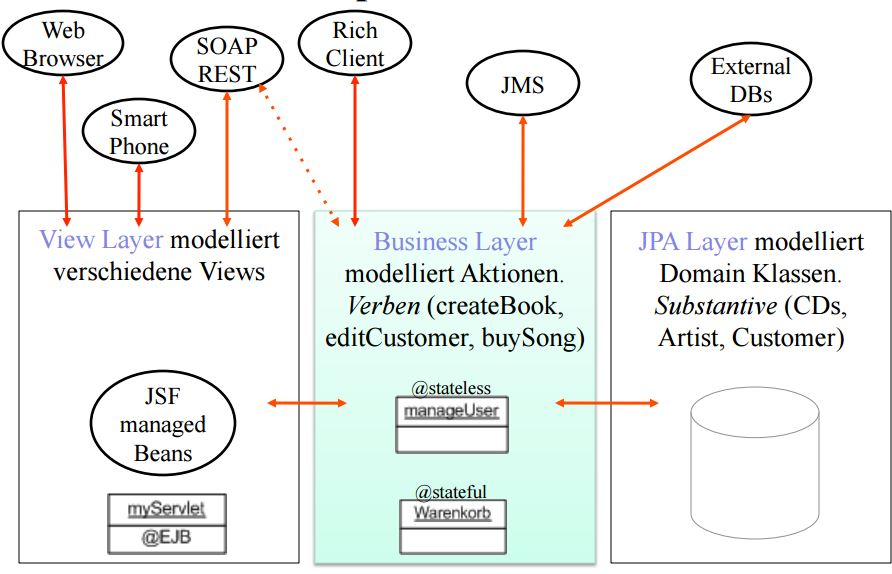
\includegraphics[width=0.7\linewidth]{fig/ejb-layering}
	\caption{EJBs in der Architektur}
	\label{fig:ejb-layering}
\end{figure}

\section{EJB Lite}
Das abgespeckte EJB. Wenn ich an EJB Lite denke, dann denke ich immer an das Zitat \emph{Leicht zu sein bedarf es wenig, und wer leicht ist, der ist König}. Die Realität hat gezeigt, dass EJBs in der voll umfänglichen Leistungsspanne nicht immer benötigt werden. Man musste aber immer EJB in der ganzen Pracht verwenden - das führte dazu, dass sich Entwickler oft mit technischen Aspekten befassen musste, welche für sie eigentlich völlig irrelevant sind und Systeme unnötig verkomplizierten. Dazu wurden mit dem JSR 316 sogenannte Profile eingeführt, welche typische Anwendungsfälle abdecken (z.B. Webapplikation). Nun gibt es im EJB das Profile EJB Lite, welches eine Untermengen aller EJB Technologien repräsentiert. Wobei der Fokus auf Webapplikation liegt - ohne eine aufwendige Mittelschicht. Hier brauchen wir oft keine Rmeote-Zugriffe, EJB Timer oder Message Driven Beans. Funktionalitäten wie DI, Persistenzabbildung, Session Beans und deklarative Transaktionssteuerung genügen.

\section{EJB-Typen}
Es gibt grundsätzlich drei Typen von EJBs:
\begin{description}
	\item[Session Bean:]
		Sessions Beans sind für gewöhnlich eine nicht persistente, serverseite Komponenten, in der die Logik Geschäftsprozesses implementiert wird. Solche Beans können über Webservice-Schnittstellen zur Verfügung gestellt werden und ermöglichen schnelle Integrationsmöglichkeiten in Umsystemen. Diesen Typ von Bean gibt es in drei Ausprägungen:
		\begin{description}
			\item[Stateless Session Bean:] Bleibt dem Client nur für die Dauer des Methodenaufruf zugeordnet. Nachdem die Verarbeitung beendet ist, ist diese Bean auch wieder für andere Clients nutzbar. Die Klasse muss mit \verb|@Stateless| annotiert werden.
			
			\begin{figure}[h!]
			\centering
			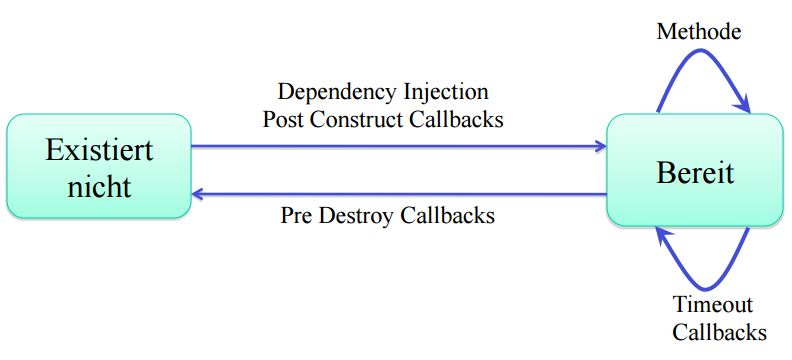
\includegraphics[width=0.5\linewidth]{fig/ejb-lifecycle-statless-bean}
			\caption{Lifecycle Stateless Session Bean}
			\label{fig:ejb-lifecycle-stateless-bean}
			\end{figure}
			
			Die instanziierten Bean stehen in einem Bean Pool zur Verfügung (bean pooling). Statless Bean bedienen mehrere Clients und sind so einfacher in der Handhabung und können wiederverwendet werden (scalibility). Container müssen keine Beans dieser Art von RAM auf die Festplatte auslagern (performance).
			
			\item[Statefull Session Bean:] Bleibt dem Client der sie angefordert hat solange zugeordnet, bis dieser sie wieder freigibt. Eine Instanz einer Bean ist also einem Client exklusiv zugeordnet. Dies ermöglicht, dass ein Zustand innerhalb des Beans für den Client gespeichert werden kann. Die Klasse muss mit \verb|@Statefull| annotiert werden.
			
			\begin{figure}[h!]
			\centering
			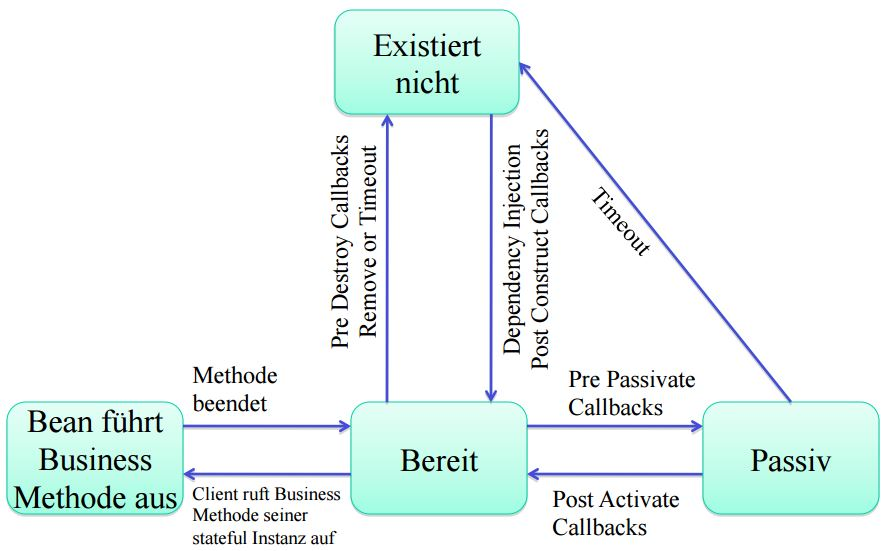
\includegraphics[width=0.5\linewidth]{fig/ejb-lifecycle-statefull-bean}
			\caption{Lifecycle Statefull Session Bean}
			\label{fig:ejb-lifecycle-statefull-bean}
			\end{figure}
			
			\item[Singleton Session Bean:] Pro JVM wo der Applikationsserver läuft gibt es maximal eine Instanz. Diese kann allerdings von mehreren Clients gleichzeitig verwendet werden. Dieser Typ eignet sich für die applikationsweit gültige Informationen.Die Klasse muss mit \verb|@Singleton| annotiert werden.
		\end{description}
	
	\item[Message Driven Bean:] Eine Message-Driven Bean (MDB) wird für die Implementierung asynchroner Kommunikation in Java-EE-basierten Systemen eingesetzt. Diese kann ausschliesslich auf indirektem Weg über Nachrichten angesprochen werden. Kein Client kann direkt Methoden einer MDB aufrufen. Eine MDB nimmt Nachrichten von einem \emph{Message-Broker} entgegen und stellt somit einen Nachrichtenendpunkt dar. Message Driven Beans sind immer \emph{stateless}. Grundsätzlich kann man sagen, dass MDBs eher technische als fachliche Komponente darstellen. Sie delegieren die Aufgaben dann oft an die entsprechenden EJBs. Muss mit \verb|@MessageDriven| annotiert werden.
	
	\item[Entity Beans:] Sind seit EJB 3.x nicht mehr relevant. Diese repräsentierten Daten, welche vollständig vom Container verwaltet wurden. Heute verwenden wir das Java Persistence API (JPA) - siehe unten Persistent Entity.
		
	\item[Persistent Entity:] Ist ein leichtgewichtiges Domänenobjekt. Es repräsentiert eine Objektsicht auf persistente und in der Regel fachliche Daten. Wird daher eigentlich nicht als EJB-Typ gezählt!
\end{description}

\section{Aufrufmodelle}
Es gibt drei Aufrufmodelle.

\begin{description}
	\item[Aufrufmodell Remote (entfernt):] Kommt immer zum Einsatz, wenn EJB Komponenten über Rechner- und/oder Prozessgrenzen hinweg angesprochen bzw. genutzt werden sollen. Es gibt diverse Motivationen dafür: Lastverteilung, Performanzsteigerung, fachliche Dekomposition sowie Aggregation/Komposition von Komponenten aus unterschiedlichen fachlichen Kontexten zu neuen (virtuellen) Applikationen. Die Komponenten können dabei über Namensdienste im Netzwerk gefunden werden - die EJBs selber werden dann über RMI aufgerufen. Mit EJB 3.1 können Methoden dabei sowohl synchron wie auch asychron aufgerufen werden. Das EJB, welches remote aufgerufen werde kann, muss mit \verb|@Remote| annotiert werden. Dies kann im EJB oder auch in der Geschäftsschnittstelle erfolgen. Die Daten werden mit Semantik \emph{by value} übergeben (serialisiert, deseralisiert). Der Empfänger erhält keine Referenzen sondern Kopie der Originaldaten.
	
	\item[Aufrufmodell Local (lokal):] Dieses sollte so häufig wie möglich eingesetzt werden. Denn es ist das performanteste. Jedoch müssen die Komponenten im selben Prozessraum sein. Auch hier ist sowohl synchron wie auch asynchrone möglich. Dafür muss die Annotation \verb|@Local| auf dem Bean deklariert werden. Diese Annotation kann aber auch weggelassen werden, denn diese ist die voreingestellte Zugriffsart.
	Seit EJB 3.1 kann die Angabe eines Interface für lokale Zugriffe ganz entfallen. Falls eine Session Bean kein Interface implementiert und keine lokale oder entfernte Schnittstelle definiert, dann erhält diese Bean automatisch eine sogenannte \emph{No-Interface Client View} - eine lokale Schnittstelle mit allen als public deklarierten Methoden der Bean. Diese Client View kann auch explizit über die Annotation \verb|@LocalBean| deklariert werden. Die Parameter werden mit der Semantik \emph{call by reference} übergeben (jaja - wir wissen, dass Java immer call by value ist!). 
	
	\item[Aufrufmodell Nachrichtenbasiert:] Zu guter Letzt gibt es noch das nachrichtenbasierte Aufrufmodell, welches mit dem EJB-Typ MDB mit hergeht. Die Kommunikation erfolgt immer über einen Brocker und ist immer asynchron. Man kann folgendes entkoppeln: Ganze Systeme, Klassen, Komponenten, fachliche Domänen innerhalb von Systemen. Und ein wichtiger Punkt ist die Integration von Legacy-Systemen.
\end{description}

\section{Dependency Injection vs. JNDI Lookup}
Beide machen technisch das genau gleiche. Aber die Dependency Injection ist um einiges eleganter und koppelt lose. Die Dinge werden injiziert und die Klasse selber muss sich nicht darum kümmern mittels eine JNDI Lookup mit try/catch Blöcken usw.

\section{Methoden-Typen in EJBs}
Schlussendlich sind die EJBs nichts anderes als POJOs. In der Praxis werden Business-Methoden in einem Interface definiert, welches das Bean implementiert. Zudem gibt es sogenannte Lebenszyklus oder auch Callback-Methoden. Diese werden vom Container aufgerufen \emph{Don't call us - we'll call you. Hollyword-Prinzip.}. Es gibt beispielsweise \verb|@PostConstruct| oder \verb|@PreDestroy|. Bei Statefull-Session Beans auch \verb|@PostActivate| oder \verb|@PostPrePassivate|. Auch die persisten Entities haben Callback Methoden, die werden aber meiner Meinung nach nicht vom Container aufgerufen sondern vom \verb|EntityManager|.

\section{Kontexte}
Das Interface \verb|javax.ejb.EJBContext| stellt die Informationen, welche vom Container verwaltet werdern zur Verfügung. Wichtige Methoden darin: \verb|getCallerPrincipal()|, \verb|isCallerInRole()|, \verb|lookup|. Das Interface wird von drei weiteren Interfaces erweitert, welche spezifisch für die Bean-Typen sind:
\begin{description}
	\item[javax.ejb.SessionContext:] Definiert den Kontext für Session Beans. Beinhaltet einige weitere Methoden.
	
	\item[javax.ejb.MessageDrivenContext:] Dieser Kontext ist speziell für die MDBs. Dieses Interface spezifiziert keine weiteren Methoden.
	
	\item[javax.ejb.EntityContext:] Kontext für die veralteten Entity-Beans. Hat beispielsweise die Methode \verb|getPrimaryKey()| enthalten. Gutes Indiz dafür, dass der Container die Entity-Beans wirklich gemanaged hat!
\end{description}

\section{EJB-Container}
Der EJB-Container ist ein Element innerhalb des Java-EE-Applikationsserver. Er beherbergt Instanzen von EJB-Komponenten und ermöglicht und überwacht deren Ausführung. Die dazu benötigten Funktionen stellt er selber zur Verfügung oder fordert diese vom App-Server an.

\begin{itemize}
	\item Früher hat beispielsweise der EJB-Container sich auch noch um das Persistenzmanagement gekümmert mit den Entity Beans, da wird aber heute mittels JPA gelöst.
	\item Eine wichtige Sache ist aber das \textbf{Transaktionsmanagement}.  Die Nutzung davon kann deklarativ wie auch programmgesteuert erfolgen.
	\item Zudem muss er den \textbf{Lebenszyklus von EJBs} steuern.
	\item Auch die \textbf{Zugriffsrechte} müssen durch den Container gemanaged werden.
	\item Er führt \textbf{Instanz-Pools} von EJBs.
	\item Der Container isoliert die Klasse mit der Implementation von ihrem Client (Aufrufer). Clients müssen einen Aufruf durch OJBObject in den Container machen.
	\item Der Container stellt Timer Zeit Services zur Verfügung die es erlauben eine Methode zu einer bestimmten Zeit aufzurufen.
	\item Für Message-Driven Beans überwacht der Container eine Message Queue im  Auftrage der EJB Komponente. 
	\item Concurrency Support 
\end{itemize}

\section{EJB Timer Service}
Im Unix kennn wir doch alle das Programm cron. Ein anderes Scheduling System bietet uns der EJB-Container. EJBs können nämlich den Timer Service verwenden. Timer Events können zu folgenden Zeitpunkten ausgeführt werden:
\begin{itemize}
\item Zu einer bestimmten Zeit 
\item Nach einer bestimmten verstrichenen Zeit 
\item An bestimmten, sich wiederholenden Zeitintervallen 
\end{itemize}	

Der EJB Timer Service ist nur für Stateless Session Beans, Singleton Session Beans und Message-Driven Beans gedacht. In Statefull kann dieser nicht verwendet werden. Da diese in der Regel eher einen kurzen Zeitraum einer Client-Session einen Zustand besitzen und Timer Service aber primär für lange laufende, zeitgesteuerte Aufgaben konzipiert ist.

\section{Asynchroner Bean Call}
Annotiere die Methode mit \verb|@Asynchronous| und der Methoden-Aufruf kehrt direkt zurück.

\section{Proxy Modell}
Der Container gibt beim Aufruf einer Session Bean an den Client nur immer einen Stellvertretter (Proxy) zurück. Der Client arbeitet mit dem Stub und auf dem Server ist der Skeleton.

\section{Client Zugriff auf Beans}
Die Typen eines Clients sind local, remote oder Web Service. Wobei der local Client in der gleichen JVM laufen muss, kann eine Web-Komponente oder ein anderes EJB sein. Vom lokalen Client ist die Lokalität des Beans auf das er zugreift, nicht transparent. Ausserhalb der JVM muss immer über das Remote-Interface zugegriffen werden. Welches soll ich wählen - falls unsicher wähle remote (bin nicht dieser Meinung).

\newpage
\section{Naming Convetions}
\begin{figure}[h!]
\centering
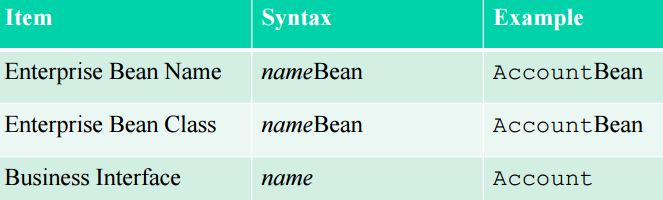
\includegraphics[width=0.7\linewidth]{fig/ejb-naming-convention}
\caption{EJB Naming Convention}
\label{fig:ejb-naming-convention}
\end{figure}

\section{Servlet ruft Bean an}
Servlets können frei nach belieben stateless und stateful Session Beans aufrufen. Der Entwickler sollte jedoch folgende Regeln beachten: Servlets sollten keine Entitätsklassen aufrufen (direkten DB Zugriff), denn die Beschränktheit der
Transaktionsgrenzen führt zu ineffizienten Synchronisationen. Servlets sollten nur wenige (dafür komplexe) anstatt viele einfache Methodenaufrufe machen (reduziert RMI Overhead). Stateless Session Beans können zur Initialisationszeit (Servlets) lokalisiert werden, denn JNDI Lokalisierungen sind aufwendige Operationen 

\section{Kontrollfragen}

\subsection{Welche Arten von Enterprise Bohnen Kennen Sie?}
\begin{itemize}
	\item Session Beans (Stateless, Statefull, Singleton)
	\item Message Driven Beans
\end{itemize}
Wir kennen noch die veralteten Entity Beans, welche durch die persistent Entity abgelöst wurden. Die persistent Entity sind aber keine EJBs.

\subsection{Welche Eigenschaften besitzen die Sessions Beans?}
\begin{description}
	\item[Stateful:] Sie bestehen während einer User-Session. Pro User-Session gibt es pro Bean nur eines.
	\item[Stateless:] Es gibt viele, sie werden dynamisch aus einem Pool verwendet. 
	\item[Singleton:] Es wird nur einmal pro Applikation instanziiert. Stellen globalen, einmaligen Zugriffspunkt dar.
\end{description}

\subsection{Welche 2 Methodenarten können in einem EJB implementiert werden?}
\begin{description}
	\item[Business Methoden:] Werden vom Entwickler programmiert.
	\item[Lebenszyklus / Call-Back Methoden:] Stellt der Container zur Verfügung. 
\end{description}

\subsection{Auf welche Art greift ein Client auf ein Bean zu?}
Der Zugriff kann wie folgt erfolgen: Remote, Locale oder WebService.

\subsection{Brauchen alle Beans ein Interface?}
Nein, seit Java EE 6 können auf Beans via der impliziten Local Interface View zugegriefen werden.

\subsection{Kann ein Rich-Client auf ein Bean mit „local“ definiertem Interface zugreifen?}
Rich-Client: Java Applikation die lokal auf einem Notebok, z.B. Swing-Application
Nein, muss mindestens Remote deklariert sein.

\subsection{Wieso haben Beans eine spezielle Namenskonvention?}
Damit sie geordnet und schneller gefunden werden können.

\subsection{Wie viele ... ?}
@Stateful: 1
@Stateless: so viele wie nötig

\subsection{Wann wird eine Annotation ignoriert?}
Wenn es im XML-File übersteuert wird. (XML hat die höhere Priorität!)

\subsection{Wenn sie zur Laufzeit etwas vom Container wissen/verwenden möchten, wie machen Sie das?}
Ich greife auf die Kontexte zu: EJB Context, Session Context, Message Driven Context.

\subsection{Wie nennt man die Beans wo man im Web-Tier am besten eine Referenz auf eine Session Bean macht?}
Managed Beans (auch Backing-Bean genannt)
